\subsection{Математическое моделирование}

\subsubsection{Модель ``Hybrid Stepper Motor'' из пакета ``SimPower Systems''}

Для моделирования процессов, протекающих в системе, воспользуемся пакетом MATLAB.
Перед построением модели всей системы, необходимо получить все параметры,
необходимые для использования встроенной модели гибридного шагового двигателя из пакета:

\textit{SimPower Systems -> Second Generation -> Motors and Generators -> Hybrid Stepper Motor}.

Известно всё необходимое, за исключением величины потосцепления, формируемого
постоянными магнитами ротора. Его можно определить по формуле
из \cite{Matlab_help_stepper_motor}:

\begin{equation}
    \label{maximum_flux_linkage}
    \psi_{M} = \frac{30}{\pi N_{r}} E_{M} n
\end{equation}

где $n$ - частота вращения ротора, об/мин

$E_{M}$ - амплитудное значение ЭДС самоиндукции разомнутой обмотки статора, В
\vspace{\baselineskip}

Число пар полюсов двигателя:
$$
N_{r} = \frac{360}{2m \cdot step} = 50
$$

где $m = 2$ - число фаз шагового двигателя,

$step = 1,8$ - шаг углового перемещения шагового двигателя, град

Для использования (\ref{maximum_flux_linkage}) проведём следующий эксперимент:
с помощью дополнительного двигателя на стенде разгоним интересующий нас шаговый
двигатель до частоты вращения $n = const$ и с помощью осцилографа определим $E_{M}$
в одной из его разомкнутых обмоток.

\subsubsection{Модель в ``MATLAB Simulink''}
Обозначим процессы, модерируемые в работе привода на созданной модели:

\begin{itemize}
    \item Токовые контуры в обмотках двигателя
    \item Сухое и вязкое трение
    \item 3 среднечастотных резонансных гармоники (см. \cite{Novel_Modeling_and_Damping})
\end{itemize}

В созданной модели используется следующие допущения:

\begin{itemize}
    \item Пусть момент двигателя пропорционален току, то есть пренебрежем той частью переходных
            процессов, где это не так
\end{itemize}

\paragraph{Токовые процессы}
Для контура одной фазы двигателя, пренебрегая наличием ёмкости внутри обмоток, можно записать
закон Ома:

Для фазы A:
\begin{equation}
    \frac{di_{a}}{dt} =
        - \frac{R}{L_{0}} i_{a}
        + \frac{K_{M}}{L_{0}} \omega_{p} \sin(N_{r}\theta)
        + \frac{\vartheta_{A+} - \vartheta_{A-}}{L_{0}}
\end{equation}

Для фазы B:
\begin{equation}
    \frac{di_{b}}{dt} =
        - \frac{R}{L_{0}} i_{b}
        - \frac{K_{M}}{L_{0}} \omega_{p} \cos(N_{r}\theta)
        + \frac{\vartheta_{B+} - \vartheta_{B-}}{L_{0}}
\end{equation}

\begin{figure}[ht!]
    \centering
    \includegraphics[width=0.8\textwidth, keepaspectratio]
                    {./src/pictures/drive_model/drive_model_current_equation}
    \caption{Реализация физики электрических процессов фазы шагового двигателя в модели}
    \label{pic_drive_model_current_equation}
\end{figure}

\paragraph{Уравнения для момента}
Будем считать, что момент пропорционален току в некотором рабочем диапазоне. Тогда можно записать:
$$
    \tau_{a} = - K_{M} i_{a} \sin({N_{r} \theta})
$$
$$
    \tau_{b} = K_{M} i_{b} \cos({N_{r} \theta})
$$
Запишем суммарный момент как сумму двух вышеописанных составляющих:
\begin{equation}
    \tau = K_{M} [-i_{a} \sin({N_{r}\theta}) + i_{b} \cos({N_{r}\theta})]
\end{equation}

\paragraph{Диссипативные силы}
В модели учитывается две составляющие трения - вязкое и сухое.

Вязкое трение аппроксимировано до составляющей, пропорциональной первой производной от угла поворота:
\begin{equation}
    \tau_{\text{тр.вязк}} = D_{\text{тр.вязк}} \cdot \omega_{p}
\end{equation}

Сухое трение получено из формулы:
\begin{equation}
    \tau_{\text{тр.сух}} = \begin{cases}
         |\tau| \cdot \frac{\omega_{p}}{|\omega_{p}|}, & \text{если} ~|\tau|  <  D_{\text{тр.сух}}, \\[2mm]
         D_{\text{тр.сух}}  \cdot \frac{\omega_{p}}{|\omega_{p}|}, & \text{если} ~|\tau| \ge D_{\text{тр.сух}}
    \end{cases}
\end{equation}

\begin{equation}
    \tau_{\text{тр}} = \tau_{\text{тр.вязк}} + \tau_{\text{тр.сух}}
\end{equation}

\begin{figure}[ht!]
    \centering
    \includegraphics[width=0.7\textwidth, keepaspectratio, clip=true, trim=25mm 35mm 25mm 35mm]
                    {./src/pictures/drive_model/drive_model_friction}
    \caption{Реализация диссипативных сил в модели}
    \label{pic_drive_model_friction}
\end{figure}

\paragraph{Среднечастотная нестабильность}
Согласно \cite[ф-ла 5]{Novel_Modeling_and_Damping}, можно выделить три основных (1-ую, 2-ую, 4-ую)
гармоники среднечастотной нестабильности.
\begin{equation}
    \tau_{\text{рез}} =   K_{d1} \cdot \sin{ (  N_{r} \theta + \phi_{1}) }
                         + K_{d2} \cdot \sin{ (2 N_{r} \theta + \phi_{2}) }
                         + K_{d4} \cdot \sin{ (4 N_{r} \theta + \phi_{4}) }
\end{equation}

где $K_{d1}$ - амплитуда первой гармоники резонанса момента

$K_{d2}$ - амплитуда второй гармоники резонанса момента

$K_{d4}$ - амплитуда четвертой гармоники резонанса момента

$\phi_{1}$ - фаза первой гармоники резонанса момента

$\phi_{2}$ - фаза второй гармоники резонанса момента

$\phi_{4}$ - фаза четвертой гармоники резонанса момента

3-ья, 5-ая и более высокие гармоники оказывают незначительное влияние, а потому
ими можно и нужно пренебречь.
